% Intended LaTeX compiler: xelatex
\documentclass[koma,a4paper,utopia,10pt,listings-color,microtype,paralist,colorlinks]{org-article}
               \usepackage{tikz}
\author{Eason}
\date{\today}
\title{make STEAM clear}
\hypersetup{
 pdfauthor={Eason},
 pdftitle={make STEAM clear},
 pdfkeywords={},
 pdfsubject={},
 pdfcreator={Emacs 26.3 (Org mode 9.2.6)},
 pdflang={English}}
\begin{document}

\maketitle
\tableofcontents



\section{Videos}
\label{sec:org002a437}



\section{Posts}
\label{sec:org2d95323}



\subsection{Set up the TikZ in Emacs Org File}
\label{sec:org64c90ff}
\begin{summary}
Why is this in \textbf{green}?
\end{summary}

\subsubsection{config the header args}
\label{sec:org825d7de}


You can embed TiKz (One of \(\LaTeX\) graphic package) code into a Org file. With
org-babel, you can generate ,insert and export the figure generated from Tikz
package. At first, you need set up the environment. \href{https://orgmode.org/worg/org-contrib/babel/languages/ob-doc-LaTeX.html}{This Post} serves as a good
introduction for beginners. Following it you may have a minimum working example
like below:

\begin{verbatim}
#+name: tutorial
#+header: :file "~/Dropbox/mstemc_hugo/static/img/tikz/tutorial.png"
#+header: :results raw :exports none :fit yes :border 0cm
#+header: :imagemagick t :iminoptions -density 400 :imoutoptions -geometry 400 -flatten
#+header: :headers '("\\usepackage{tikz} \\usetikzlibrary{positioning, shapes.symbols, calc}")
#+begin_src latex
  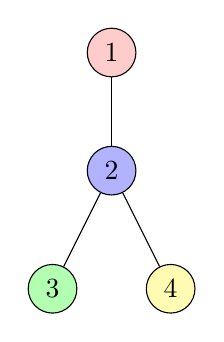
\begin{tikzpicture}
    \node [circle, draw, fill=red!20] at (0,0) {1}
    child { node [circle, draw, fill=blue!30] {2}
      child { node [circle, draw, fill=green!30] {3} }
      child { node [circle, draw, fill=yellow!30] {4} }};
  \end{tikzpicture}
#+end_src
#+RESULTS: tutorial
[[file:../../img/tikz/tutorial.png]]
\end{verbatim}

The example begins with several lines containing \texttt{\#+header} which is sort of
clutter. we can put them in a file and include it at the beginning of the Org
file.
\subsubsection{generate results with different formats}
\label{sec:org75935d2}


By changing the extension of \texttt{:file} (which is \texttt{pdf} for
\texttt{"../../img/tikz/tutorial.pdf"} ), we can generate results with different formats.
Now, I need \texttt{pdf} and \texttt{png} . You can see the result by just press \texttt{C-c C-c} in the
body of the tikz code.
\subsubsection{export the results according to the backend}
\label{sec:org59da2c2}


You can set \texttt{:exports} to control how the results will be exported. Now I set it
as \texttt{none} which means the result will not be exported to latex or other format. I
want to set more options of the exports. So I use:

\begin{verbatim}
#+ATTR_HTML:  :width 800 :align center
#+ATTR_LATEX: :width 0.8\textwidth :align center
{{{if-latex(tutorial.pdf,tutorial.png)}}}
\end{verbatim}

\texttt{if-latex} is a Org MACRO whose definition is :
\begin{verbatim}
#+MACRO: if-latex (eval (if (org-export-derived-backend-p org-export-current-backend 'latex)
 (concat "[[file:../../img/tikz/"  $1 "]]")
 (concat "[[file:../../img/tikz/"  $2 "]]") ))
\end{verbatim}

The \texttt{if-latex} MACRO let you export different formats by the backend. If the
backend is \texttt{latex} then, \texttt{pdf} format figure will be exported. Otherwise, \texttt{png} format
figure. Eventually, in the final \texttt{pdf} document, you figure can be zoomed in or
out without losing any resolution.

\subsubsection{the final workflow}
\label{sec:orgc0cd8cc}


The minimum working example at the start of this post is simplifed as below.

\begin{verbatim}
#+header: :file  "../../img/tikz/tutorial.pdf"
#+begin_src latex
  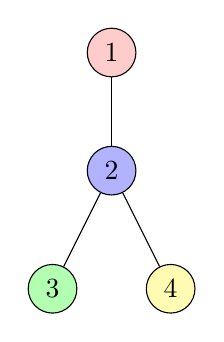
\begin{tikzpicture}
    \node [circle, draw, fill=red!20] at (0,0) {1}
    child { node [circle, draw, fill=blue!30] {2}
      child { node [circle, draw, fill=green!30] {3} }
      child { node [circle, draw, fill=yellow!30] {4} }};
  \end{tikzpicture}
#+end_src

#+RESULTS:
[[file:../../img/tikz/tutorial.png]]

The following is the generated figure.
#+ATTR_HTML:  :width 800 :align center
#+ATTR_LATEX: :width 0.8\textwidth :align center
{{{if-latex(tutorial.pdf,tutorial.png)}}}
\end{verbatim}

Many settings are grouped into a setup file which is included at the top of this
post:
\begin{verbatim}
#+SETUPFILE: ~/.spacemacs.d/org-templates/math-en.org
\end{verbatim}

Now, If you set the extension of the target file in the first line either \texttt{pdf} or
\texttt{png} , a corresponding \texttt{pdf} or \texttt{png} figure will be generated. If execute \texttt{M-x
org-toggle-inline-images}  , you can preview the result. If export the org-file
as latex file then the \texttt{pdf} file, the image of \texttt{pdf} format will be inserted. If
export to other format, \texttt{png} image will be used.


\section{Projects}
\label{sec:org8f61cb8}


\subsection{my workflow of creating a video}
\label{sec:org597f5bb}
During the creation of one video, several tools are tuned to fit my workflow. In
this project several videos and posts will be created to make my workflow clear.

Two targets of this project:
\begin{enumerate}
\item remind me of the configuration of several tools;
\item show somebody else who may be interested in how I work.
\end{enumerate}

I am not ready to detail each tool. If you are interested in any one of them,
please refer to tutorials written by experts or given by the official document.

\subsubsection{Emacs}
\label{sec:org76d34e1}


Emacs lies in the center of my workflow. It behaves like a super-IDE which
assists me finish almost all the steps. Using Emacs, I program and debug, GTD,
write the blogs, export and publish them. Many of the Emacs extensions are
awesome. In particular, Emacs Org is the killer app.

How to config Emacs? After more Than ten years of using Emacs, I choose
spacemacs. Most beginners can start their work using spacemacs with only a
little modifications.

\begin{enumerate}
\item program and debug
\label{sec:orgd2ab070}


I program in python, C/C++, Matlab and some other languages. Emacs acts as a
super-IDE for me.


\item Org mode - journalize your work
\label{sec:org75ff6e1}


Org mode definitely need a standalone subsection.

\item Org mode - get things done
\label{sec:org4df4183}



\item Org mode - write a diary
\label{sec:org266bdcc}

\item Org mode - export your Org file
\label{sec:orge9ee370}


\item program and debug
\label{sec:orgcf10226}


\item writing latex
\label{sec:org69631c2}
\item org-journal
\label{sec:org06a8ebe}


I write many notes during a post or a project. Most of my journal is maintained
by \href{https://github.com/bastibe/org-journal}{org-journal: A simple org-mode based journaling mode} . And I set the
\texttt{org-journal-file-type} to \texttt{weekly} So that I have around 52 journal file each
year.

The journals can be searched conveniently. Also they can be integrated into Org
agenda.


\item ox-hugo
\label{sec:orgde97df4}


\href{https://github.com/kaushalmodi/ox-hugo}{kaushalmodi/ox-hugo: A carefully crafted Org exporter back-end for Hugo}

Because hugo supports markdown at first (it also supports org file later), I use
Emacs Org from the very beginning. I am quite familiar with org-mode, so have no
motivation to dig into markdown. Fortunately, ox-hugo meets all my requirement
and definitely worth a try when you want to stay in Org.

Actually, Emacs have extensions to support markdown quite well. However, using
Org, I can integrate the org file into my agenda.


\item preview tikz picture in Org
\label{sec:org2bcb08b}


\href{http://www.texample.net/tikz/}{TikZ and PGF} are \TeX{} packages for creating graphics programmatically. TikZ is
build on top of PGF and allows you to create sophisticated graphics in a rather
intuitive and easy manner.

You can integrated TikZ code into the Org mode as a source block. I have a
not-so-detailed post on how to set up the tikz environment in Org.
\end{enumerate}


\subsubsection{Hugo}
\label{sec:org79f095e}


As the fastest framework for building websites, Hugo shocks me by its speed and
flexibility. It is enough to prettify your site using the more than 300+
beautiful themes, from which I am in the mode for Academic theme.

Hugo supports Org file but not so good. Ox-hugo, another extension of Emacs, has
my attention. Serving as a bridge between Emacs and Hugo, ox-hugo helps me
staying in Emacs Org. There is no need for me to write markdown file if Org is
available.

I use ox-hugo as a bridge between Emacs and Hugo. So I do not have to care much
about how to leverage Hugo. Ox-hugo helps me do most of the work.

\subsubsection{manim}
\label{sec:orga490cc3}



\subsubsection{blender}
\label{sec:org362635d}



\section{Courses}
\label{sec:orgc9e6ff6}
\end{document}
